
%Bevor die Modellbildung starten konnte, mussten zunächst die Bedingungen geklärt werden. 
%Das bedeutet, dass der Datensatz analysiert werden musste und eine entsprechende Problemstellung identifiziert werden musste. 
Im Rahmen des Praktikums wurde zuerst der Datensatz analysiert. Im Folgenden wird zunächst der ursprüngliche Datensatz beschrieben und anschließend erklärt, wie dieser im Laufe des Projekts ausgebaut und ergänzt wird. Danach wird die daraus abgeleitete Problemstellung erläutert.

\subsection{Ursprünglicher Datensatz}
\label{UrsprunglicherDatensatz}
%Erter Satz geändert
Als Basis wurden der Datensatz \cite{Urbanbricks2020} verwendet. Die Daten lagen in zwei Dateien unterteilt vor. Die erste Datei enthielt gute Artikel und die zweite enthielt %\emph{promotional} (
Werbeartikel. Die Werbeartikel haben dabei eigene Labels: advert (Werbeanzeigen), coi (enge Verbindung des Autors zum Artikel), fanpov (potentielle Fandarstellung), PR  (Presseartikel), resume (Lebenslauf).
%\begin{itemize}
%    \item advert - „Dieser Artikel enthält Inhalte, die wie eine Werbeanzeige verfasst sind.“
%\item coi - „Ein Hauptautor dieses Artikels scheint eine enge Verbindung zu seinem Thema zu haben.“
%\item fanpov - „Dieser Artikel ist möglicherweise aus der Sicht eines Fans geschrieben, statt aus einer neutralen Perspektive.“
%\item pr - „Dieser Artikel liest sich wie eine Pressemitteilung oder ein Nachrichtenartikel oder basiert weitgehend auf routinemäßiger Berichterstattung oder Sensationslust.“
%\item resume - „Dieser biografische Artikel ist wie ein Lebenslauf geschrieben.“
%\end{itemize}
%Der zweite Datensatz enthielt Artikel, die als \emph{good} klassifiziert worden sind. 
Der Datensatz zeigte erhebliche Ungleichgewichte in der Verteilung der Werbe-Labels.

\begin{figure}[H]
    \centering
    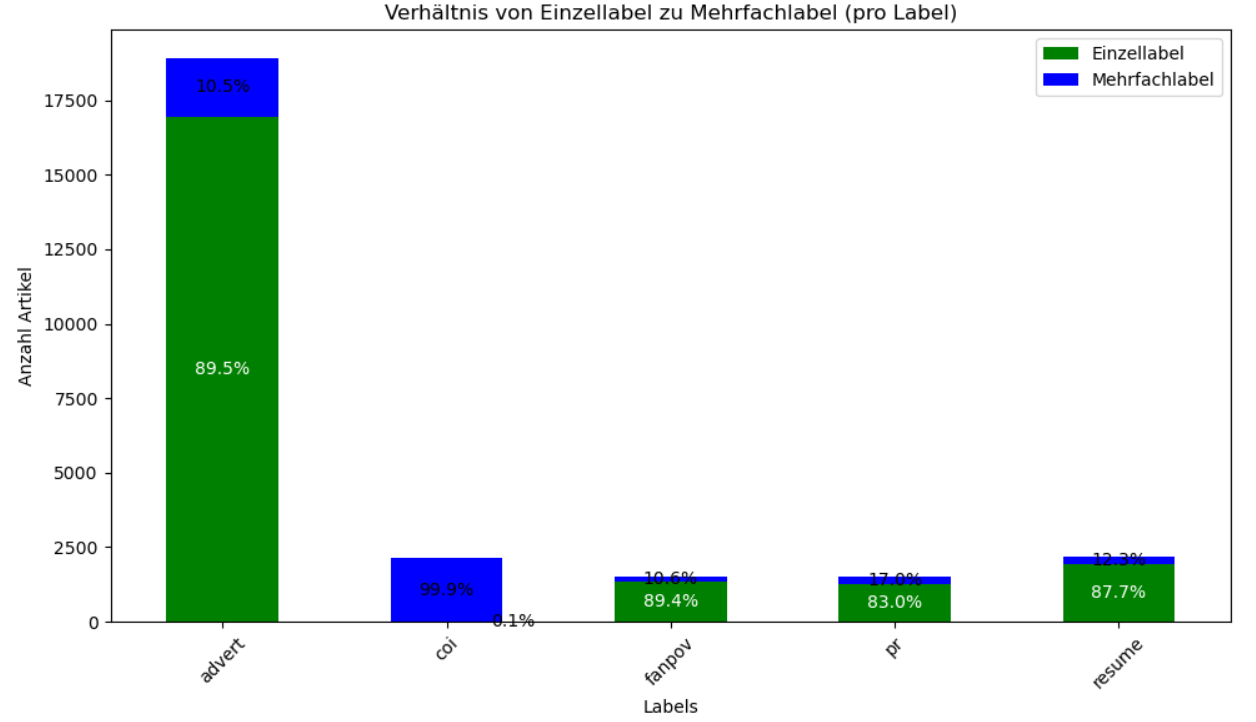
\includegraphics[width=0.7\linewidth]{figures/labelverteilung.png}
    \caption{Verteilung der Werbelabels.}
    \label{fig:labelverteilung}
\end{figure}

Wie in Abbildung \ref{fig:labelverteilung} deutlich wird, dominiert das Label advert gegenüber den anderen Labels, während insbesondere coi mit nur drei eigenständigen Labels stark unterrepräsentiert ist. Dies birgt die Gefahr, dass Modelle Schwierigkeiten haben, die weniger häufigen Werbe-Labels korrekt zu erkennen.
\subsection{Datensatzerweiterung}
\label{ProblemeDatensatz}
\label{WPDump}
Aufgrund der beschriebenen Herausforderungen mit dem Datensatz von Kaggle, wurden weitere Artikel mittels Wikipedia-Dump beschafft. Beim Wikipedia-Dump handelt es sich um einen von der Wikimedia-Foundation veröffentlichten Datensatz, der alle Wikipedia-Seiten umfasst. Der Dump der englischsprachigen Wikipedia ist unter \cite{WpDump2024} zu finden.

Da die Seiten im Dump in Wiki-Syntax vorliegen, enthalten sie auch alle von den Wikipedia-Autoren eingesetzten Vorlagen (Templates). Jeder Artikel, der von der Wiki\-pedia-Gemeinschaft als lesenswert (\emph{good}), exzellent (\emph{featured}) oder werbend (\emph{promotional}) klassifiziert wurde, enthält mindestens ein Template, anhand dessen diese Klassifizierung erkannt werden kann. Außerdem lassen sich anhand von Templates und anderen Syntax-Elementen noch diejenigen Seiten identifizieren, welche keine Artikel darstellen, beispielsweise Begriffsklärungsseiten, Umleitungen, Kategorien und Benutzerseiten.

Es wurde ein Konverter entwickelt, der die Artikel anhand der Templates auf drei Kategorien verteilt und in CSV-Dateien schreibt: In die erste Kategorie \emph{good} fallen die als lesenswert und exzellent gekennzeichneten; in die zweite Kategorie \emph{promotional} die als werbend erkannten und in die letzte Kategorie \emph{neutral} alle weiteren Artikel. Die zur Kategorisierung genutzten Templates wurden aus dem Artikeltext entfernt. Insgesamt ergab sich die folgende Aufteilung: 46.882 \emph{good}, 32.633 \emph{promotional}, 6.611.303 \emph{neutral}. Da die Klassen extrem ungleich verteilt sind, wurde anschließend noch eine gleichgroße zufällige Auswahl der Artikel jeder Klasse getroffen (Undersampling). Hierbei kam \textit{Reservoir Sampling} \cite{Vitter1985} zum Einsatz, bei dem die Elemente des Datensatzes einzeln gelesen werden, ohne dass deren Anzahl zuvor bekannt sein muss.

\subsection{Problemdefinition}
\label{Problemdefinition}
Das Ziel dieses Projekts ist die Entwicklung von Modellen zur automatisierten Klassifikation von Wikipedia-Artikeln als \emph{promotional} (werblich) oder \emph{nicht-promotional}. Dabei gab es eine Unterteilung in drei Problemarten.
\begin{itemize}
    \item Die Verwendung des ursprünglichen Datensatzes zur binären Klassifizierung
    \item Die Verwendung des Wikipedia Dump Datensatzes zur Multiklassen-Klassifizierung zwischen guten Artikeln, neutralen Artikeln und Werbenden Artikeln
    \item Eine Multilabel-Klassifizierung, welche in den werbenden Artikeln zwischen den verschiedenen Arten (advert, coi, fanpov, pr, resume) unterscheiden kann.
\end{itemize}
%Dabei wird ebenfalls klassifiziert, wie ein Artikel promotional ist, also z.B. ob er eine Werbung, ein PR-Artikel usw. ist. Wikipedia strebt nach objektiven und neutralen Inhalten; daher ist die Identifizierung von Artikeln mit werbenden Charakter von großer Bedeutung, um die sachliche Qualität der Plattform zu gewährleisten.

%\subsection{Zielsetzung}

%Die Hauptziele des Projekts sind:

%\begin{itemize} \item Entwicklung von drei klassischen maschinellen Lernmodellen und einem Deep-Learning-Modell zur Klassifikation von Wikipedia-Artikeln. \item Vergleich der Modelle anhand von Leistungsmetriken wie Genauigkeit, Präzision, Recall und F1-Score. \item Identifikation des Modells mit der besten Leistung für die gegebene Aufgabe. \end{itemize}
